\documentclass{beamer}
\usepackage[utf8]{inputenc}
\usepackage{graphicx, epsfig}
\usepackage{amsmath,mathrsfs,amsfonts,amssymb}
%\usepackage{subfig}
\usepackage{floatflt}
\usepackage{epic,ecltree}
\usepackage{mathtext}
\usepackage{fancybox}
\usepackage{fancyhdr}
\usepackage{multirow}
\usepackage{enumerate}
\usepackage{epstopdf}
\usepackage{multicol}
\usepackage{algorithm}
\usepackage[noend]{algorithmic}
\def\algorithmicrequire{\textbf{Input:}}
\def\algorithmicensure{\textbf{Output:}}
\usetheme{default}%{Singapore}%{Warsaw}%{Warsaw}%{Darmstadt}
\usecolortheme{default}
\setbeamerfont{title}{size=\Huge}
\setbeamertemplate{footline}[page number]{}

\newcommand{\bx}{\mathbf{x}} 
\newcommand{\bz}{\mathbf{z}} 
\newcommand{\by}{\mathbf{y}} 

\newcommand{\bX}{\mathbf{X}} 
\newcommand{\bZ}{\mathbf{Z}} 

\newcommand{\btheta}{\boldsymbol{\theta}} 
\newcommand{\bphi}{\boldsymbol{\phi}} 

\DeclareMathOperator*{\argmin}{arg\,min}
\DeclareMathOperator*{\argmax}{arg\,max}

%\definecolor{beamer@blendedblue}{RGB}{15,120,80}
%----------------------------------------------------------------------------------------------------------
\title[\hbox to 56mm{Deep Generative Models  \hfill\insertframenumber\,/\,\inserttotalframenumber}]
{Deep Generative Models \\ Supplementary}
\author[Roman Isachenko]{\\Roman Isachenko}
\institute[MIPT]{Moscow Institute of Physics and Technology \\
}
\date{2020}
%--------------------------------------------------------------------------------
\begin{document}
%--------------------------------------------------------------------------------
\begin{frame}
%\thispagestyle{empty}
\titlepage
\end{frame}
=======
 \begin{frame}{GatedPixelCNN (2016)}
 \begin{figure}
     \centering
     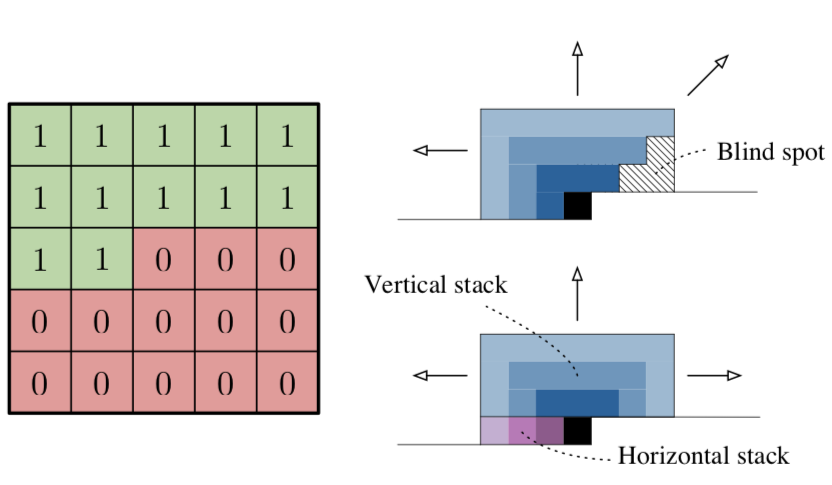
\includegraphics[width=0.5\linewidth]{figs/gatedpixelcnn.png}
     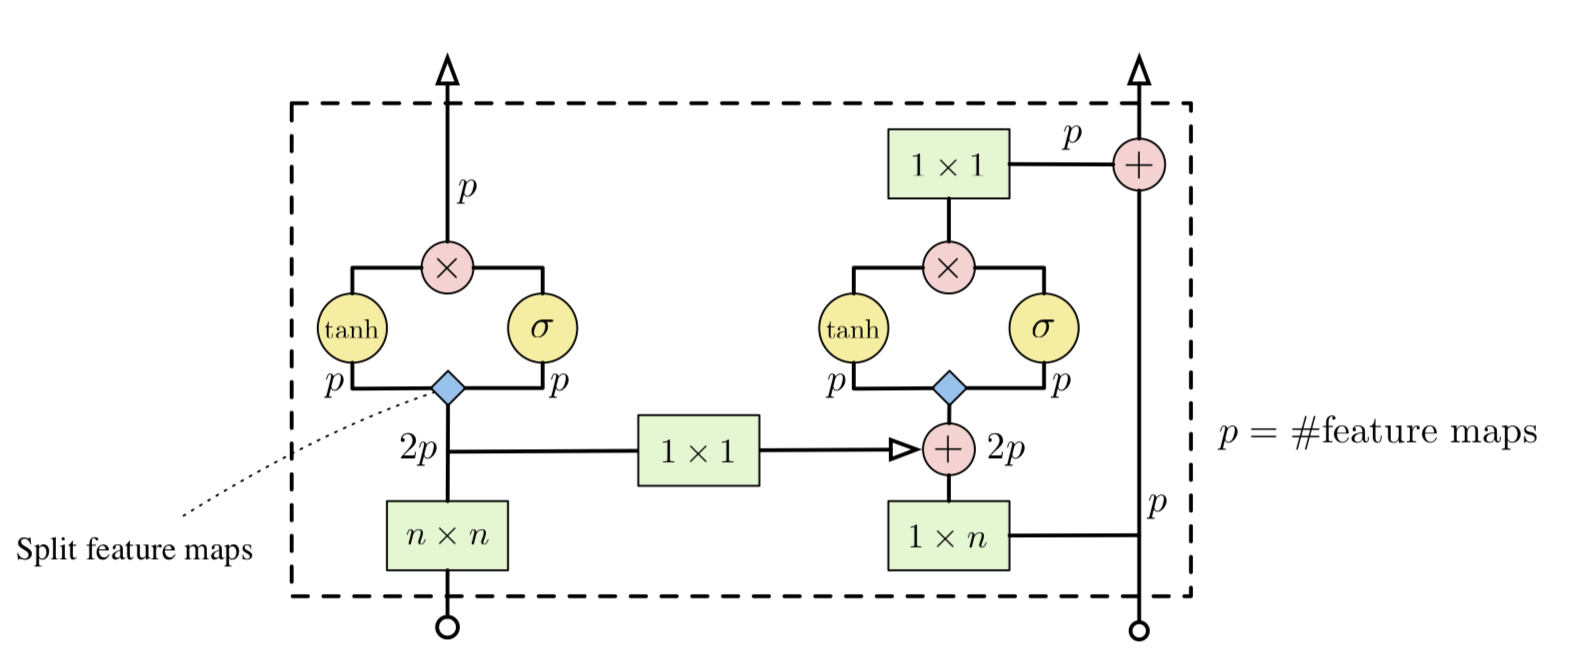
\includegraphics[width=0.5\linewidth]{figs/gated_block.png}
 \end{figure}
 \vfill
 \hrule\medskip
 {\scriptsize Van den Oord A. et al. Conditional image generation with pixelcnn decoders \href{https://arxiv.org/pdf/1606.05328.pdf}{https://arxiv.org/pdf/1606.05328.pdf}}
 \end{frame}
 %=======
 \begin{frame}{GatedPixelCNN (2016)}
 \begin{minipage}[t]{0.5\columnwidth}
 	\begin{figure}[h]
 		\centering
 		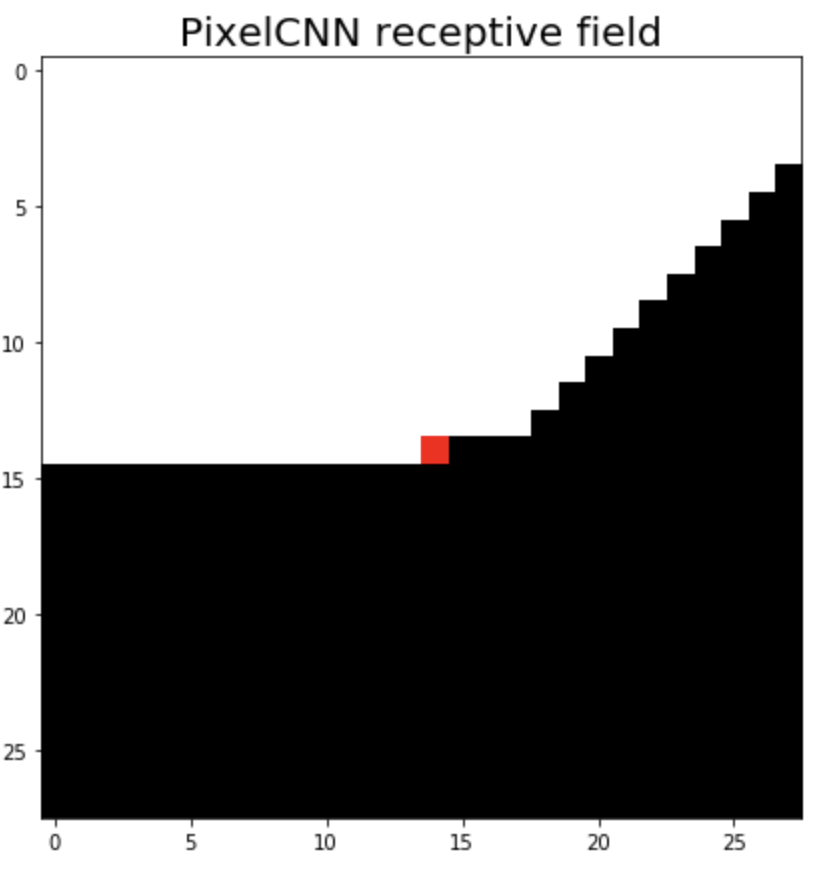
\includegraphics[width=0.9\linewidth]{figs/pixelcnn_receptive_field.png}
 	\end{figure}
 \end{minipage}%
 \begin{minipage}[t]{0.5\columnwidth}
 	\begin{figure}[h]
 		\centering
 		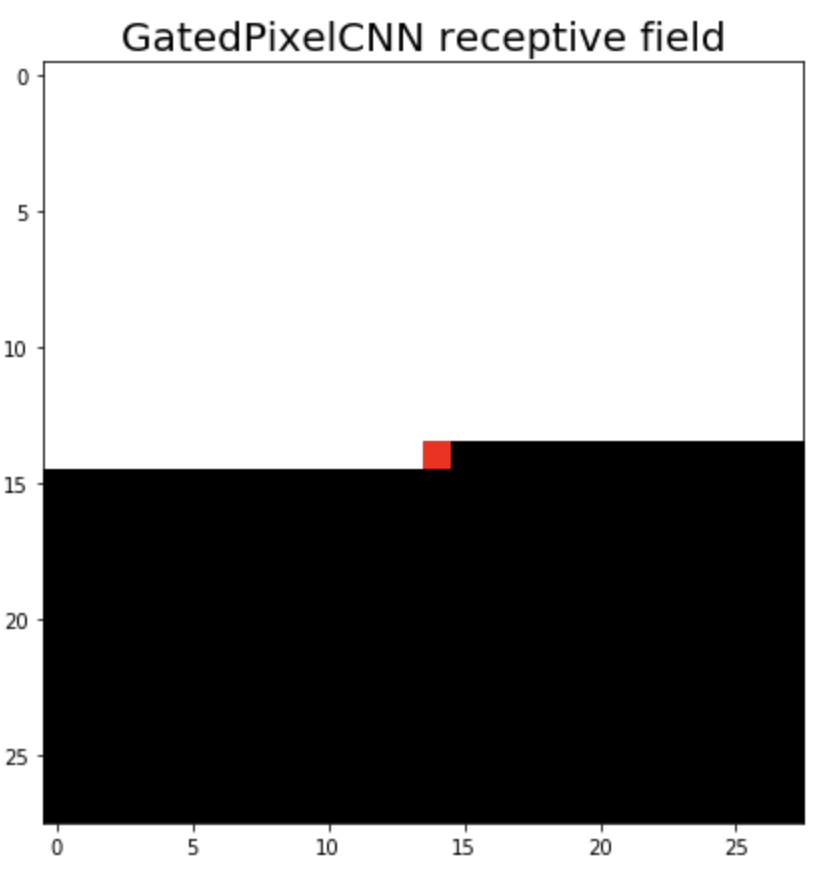
\includegraphics[width=0.9\linewidth]{figs/gatedpixelcnn_receptive_field.png}
 	\end{figure}
 \end{minipage}
 \vfill
 \hrule\medskip
 {\scriptsize Van den Oord A. et al. Conditional image generation with pixelcnn decoders \href{https://arxiv.org/pdf/1606.05328.pdf}{https://arxiv.org/pdf/1606.05328.pdf}}
 \end{frame}
 %=======
 \begin{frame}{Extensions}
     \begin{itemize}
         \item \textbf{PixelCNN++}: \textit{Improving the PixelCNN with Discretized Logistic Mixture Likelihood and Other Modifications} \\
         \href{https://arxiv.org/pdf/1701.05517.pdf}{https://arxiv.org/pdf/1712.09763.pdf} \\
         (mixture of logistics instead of softmax);
         \item \textbf{PixelSNAIL}: \textit{An Improved Autoregressive Generative Model} \\
         \href{https://arxiv.org/pdf/1712.09763.pdf}{https://arxiv.org/pdf/1712.09763.pdf} \\
         (self-attention to learn optimal autoregression ordering).
     \end{itemize}
 \end{frame}
=======
\begin{frame}{Summary}
    \begin{itemize}
        \item Sampling from autoregressive models are trivial, but sequential
        \begin{itemize}
            \item sample $x_0 \sim p(x_0)$;
            \item sample $x_1 \sim p(x_1 | x_0)$;
            \item \dots.
        \end{itemize}
        \item Estimating probability:
        \[
            p(\bx) = \prod_{i=1}^m p(x_i | \bx_{1:i - 1}).
        \]
        \item Work on both continuous and discrete data.
        \item There is no natural way to do unsupervised learning.
    \end{itemize}
\end{frame}
%=======
\begin{frame}{References}
{\tiny
\begin{itemize}
	\item \textbf{MADE}: \textit{Masked Autoencoder for Distribution Estimation} \\
	\href{https://arxiv.org/pdf/1502.03509.pdf}{https://arxiv.org/pdf/1502.03509.pdf} \\
	\textbf{Summary}: Create masked autoencoder that models autoregression (autoregression allows to make the distribution properly normalized). Sampling is performed iteratively (to generate MNIST image 784 forward passes are needed). Discrete data.
	
	\item \textbf{PixelRNN + PixelCNN}: \textit{Pixel recurrent neural networks} \\
	\href{https://arxiv.org/abs/1601.06759}{https://arxiv.org/abs/1601.06759} \\
	\textbf{Summary}: 2 models are proposed: PixelRNN, PixelCNN. The models are autoregression and sampling is sequential. For RNN two types of LSTM blocks are used: Row LSTM and DiagonalBiLSTM. CNN uses Masked convolutions. RNN outperforms, but is slower.
	
	\item \textbf{GatedPixelCNN}: \textit{Conditional Image Generation with PixelCNN Decoders} \\
	\href{https://arxiv.org/pdf/1606.05328.pdf}{https://arxiv.org/pdf/1606.05328.pdf} \\
	\textbf{Summary}: Improvements for PixelCNN: gated units (like in lstm), horizontal+vertical stacks (remove blind spots). The result is now similar to PixelRNN.
	
	\item \textbf{WaveNet}: \textit{a Generative Model for Raw Audio} \\
	\href{https://arxiv.org/pdf/1609.03499.pdf}{https://arxiv.org/pdf/1609.03499.pdf} \\
	\textbf{Summary}: Model for autoregressive audio generation, inspired by PixelCNN. Use causal convolutions for the right conditioning, and dilated atrous convolution to extend receptive field.
	
	\item \textbf{PixelCNN++}: \textit{Improving the PixelCNN with Discretized Logistic Mixture Likelihood and Other Modifications} \\
	\href{https://arxiv.org/pdf/1701.05517.pdf}{https://arxiv.org/pdf/1701.05517.pdf} \\
	\textbf{Summary}: Improved version of PixelCNN. Models mixture of logistic mixture distribution instead of softmax. Architectural modifications: skip connections, up/down sampling, dropout. Experiment with dequantization: discretization works better.
	
	\item \textbf{PixelSNAIL}: \textit{An Improved Autoregressive Generative Model} \\
	\href{https://arxiv.org/pdf/1712.09763.pdf}{https://arxiv.org/pdf/1712.09763.pdf} \\
	\textbf{Summary}: Autoregressive model. Uses masked causal convolutions. Adjust self-attention to PixelCNN.
\end{itemize}
}
\end{frame}

\end{document} 